\documentclass[a4paper]{article}

\usepackage[english]{babel}
\usepackage[utf8x]{inputenc}
\usepackage{amsmath}
\usepackage{graphicx}
\usepackage[colorinlistoftodos]{todonotes}
\usepackage{framed}
\usepackage{verbatim}
\usepackage{listings}
\usepackage{xcolor}
\usepackage{float} % para usar [H]
\lstset { 
language=C++,
backgroundcolor=\color{blue!5}, % set backgroundcolor
basicstyle=\footnotesize,% basic font setting
}

\DeclareGraphicsExtensions{.pdf,.png,.jpg, .ppm, .pgm}

\title{Tutorial, Getting Started}
\author{Imagelib}

\begin{document}
\maketitle

\begin{abstract}


\hrule
\vspace{0.5cm}
In here you can find a guide for getting stated with the imagelib library; this tutorials its actually divided in three, one for loading, creating and simple get-set functions; the next one will guide you through some basic image filtering in the spatial domain; and finally some dot to dos transformations and more.
\vspace{0.5cm}
\hrule
\end{abstract}

\section{Load, create, get, set and save images}

This tutorial will demonstrate how to load and create images, as well as handle it. Let's start loading an image from an specific directory by just calling one of the constructors of the class Image.

First you need to include the header of image lib:

\begin{lstlisting}
#include "../include/image.hh"
\end{lstlisting}

Then load the image as an Image object by passing as parameter the  location of the image(lena.ppm)

\begin{lstlisting}
Image imagen ("../../Multimedia/lena.pgm");
\end{lstlisting}

You can also create an Image object by declaring the width, height, depth, spectrum and the pixel value you want to fill the picture. In this tutorial we create an image of 256x256 with depth=1, sprectrum=3 and filled with a pixel value of 220:

\begin{lstlisting}
Image image_created (256, 256, 1, 3, 220);
\end{lstlisting}


Now that the image was created you can manage its characteristics by the sets and gets.  It is possible to get the width, height, depth, spectrum and the pixel value you want, and also set this last one:

\begin{lstlisting}
//Gets

//"__Image_object__".get_width();	    
image_created.get_width();

//"__Image_object__".get_height();
image_created.get_height();

//"__Image_object__".get_depth();
image_created.get_depth(); 
	
//"__Image_object__".get_spectrum();    
image_created.get_spectrum(); 

//"__Image_object__".get_pixel_value(x,y,z,c);
image_created.get_pixel_value(100, 150, 1, 1); 

\end{lstlisting}

All these gets return an unsigned int except the one of pixel value wich returns an unsigned char.
In this tutorial, the function set pixel value is used to set pixels with value 0. We used a scope to change only the diagonal of the image. This is how is called:

\begin{lstlisting}

//"__Image_object__".set_pixel_value(x,y,z,c,pixel value);
image_created.set_pixel_value(i, i, 1, 1, 0); 

\end{lstlisting}

The last thing to do is to save the image you created on the current directory, so just call the  save funcion like the tutorial:

\begin{lstlisting}

// "__Image_object__".save("__picture_name__");
image_created.save("image_created.ext");

\end{lstlisting}

\section{Smoothing and Sharpening Spatial Filters}

This second tutorial will guide you through the usage of smoothing and spatial filters. You can find this tutorial in the test directory of our library, in the Tutorial2.cpp file.

First, in any file that uses our library, you must include the image.hh file.


\begin{lstlisting}
# include "../include/image.hh"
\end{lstlisting}

Now we're gonna explain the rest of the code. First we create the Image object form the file, and name it parrot, the we display it.

\begin{lstlisting}
Image parrot ("../../Multimedia/parrot_original.ppm");
		
parrot.display("Parrot Original");
\end{lstlisting}

The image that we displayed will look like the one in figure \ref{parrot_original}
\begin{figure}[H]

\centering
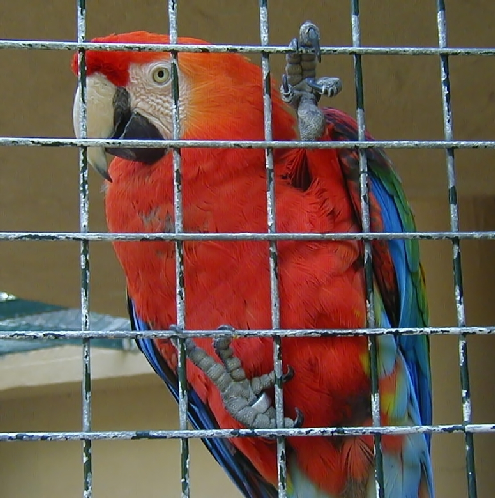
\includegraphics[scale=0.5]{./.Multimedia/parrot_original.jpg}

\caption{"Parrot Original"}
\label{parrot_original}

\end{figure}

We can apply several filters to an image. A filter returns a Image object with the corresponding filter applied to the image. For example, applying an average filter to the parrot image (it receives a int that corresponds to the intensity of the average filter. In this case its 3). Then we display it.
\begin{lstlisting}
Image smoothed_parrot = parrot.filter_average(3);
	
smoothed_parrot.display("Smoothed Parrot");
\end{lstlisting}

The result of the given filter, should look like the one on figure \ref{smoothed}

\begin{figure}

\centering
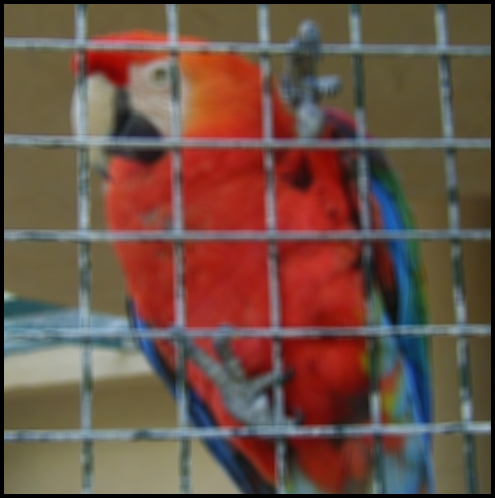
\includegraphics[scale=0.5]{./.Multimedia/smoothed_parrot.jpg}

\caption{"Smoothed Parrot"}
\label{smoothed}

\end{figure}


We can also apply a filter, and display it without storing it in a Image object. like this:
	
\begin{lstlisting}
(parrot.filter_gaussian(3,3)).display("Gaussian");
\end{lstlisting}

We can also just save the image, without storing it in an Image object like this:

\begin{lstlisting}
(parrot.filter_median(0)).save("../../Multimedia/Parrot_median.jpg");
\end{lstlisting}


The filters that we have applied are smoothing filters, that as you can see dont modify  the images alot, just, as the name says, smooth it.  Now we will apply some sharpening filters that enhance some details in the image, for example borders and noise.

We can enhance edges, by displacement. The parameters of this function are the horizontal, and vertical displacement in pixels.

\begin{lstlisting}
Image displaced = parrot.filter_edge_enhacement_displacement(1,1);
	
displaced.display("Displaced");
\end{lstlisting}

The result looks like the image on figure \ref{displaced}

\begin{figure}

\centering
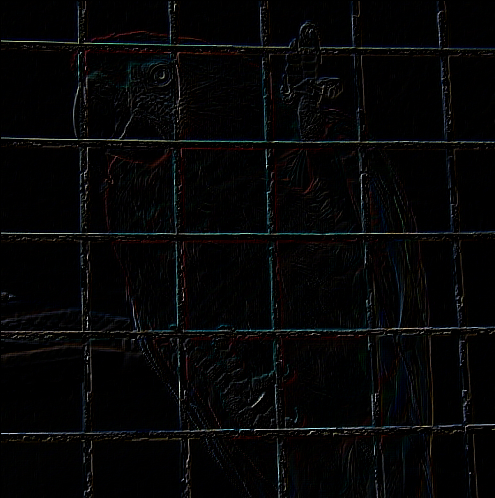
\includegraphics[scale=0.5]{./.Multimedia/parrot_displaced.jpg}

\caption{"Displaced Parrot"}
\label{displaced}

\end{figure}

We can add noise to the image, using the gaussian noise function. And apply a Laplacian filter, that acts as a sharpening filter.

\begin{lstlisting}
parrot.gaussian_noise(2);
	
Image filtered = parrot.filter_Laplacian();
	
filtered.display("Laplacian");
\end{lstlisting}

The result of this Laplacian filter looks like the image on figure \ref{laplacian}.

\begin{figure}

\centering
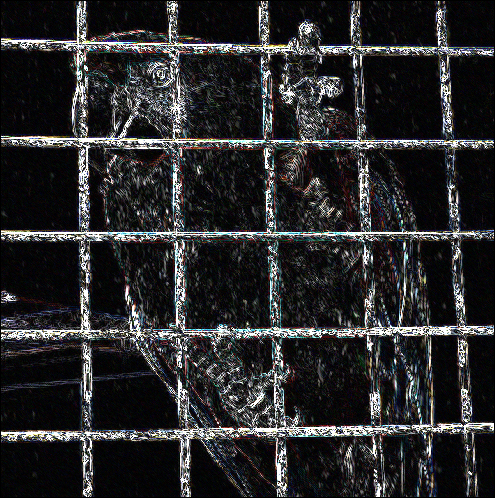
\includegraphics[scale=0.5]{./.Multimedia/parrot_laplace.jpg}

\caption{"Laplaced Parrot"}
\label{laplacian}

\end{figure}

We can overwrite an Image objec with another, in this case with a horizontal borders enhance filter:

\begin{lstlisting}

filtered = parrot.filter_horizontal_borders();
	
filtered.display("Horizontal Borders");
\end{lstlisting}

\section{Dot to Dot Transformations}

This third tutorial will guide you through the usage of dot to dot transformations. You can find this tutorial in the test directory of our library, in the Tutorial3.cpp file.


First you need to include the header of image lib:

\begin{lstlisting}
#include "../include/image.hh"
\end{lstlisting}

After that we create the Image object form the file, and name it lena, the we display it.

\begin{lstlisting}
Image lena ("../../Multimedia/lena.pgm");
		
lena.display("Lena Original");
\end{lstlisting}

The image that we displayed will look like the one in figure \ref{lena_original}
\begin{figure}[H]

\centering
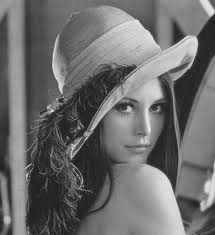
\includegraphics[scale=0.5]{./.Multimedia/lena.jpg}

\caption{"Lena Original"}
\label{lena_original}

\end{figure}

We can apply different dot to dot transformations, like the inverse function, to invert the intensity values of the pixels. To use it, first we need to create the target image object, after call the function, and we can choose if save the image or only display it. 
\begin{lstlisting}
Image lena_inverted (256, 256, 1, 1, 168);
	
lena_inverted= lena.inverse();
	
lena_inverted.save("lena_inverse.jpg");
	  
lena_inverted.display("lena inverted");
\end{lstlisting}

And the result can looks like the image on the figure \ref{lena_inverted}

\begin{figure}[H]

\centering
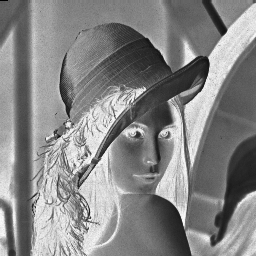
\includegraphics[scale=0.5]{./.Multimedia/lena_inverse.jpg}

\caption{"Lena Inverted"}
\label{lena_inverted}

\end{figure}

Also we can apply the dynamic range dilatation filter, is used in images poorly contrasted, and the interest is to highlight the range with more intense pixels. First we create the target image, after apply the filter, and save or display the result. This function recives two unsigned char that represents the cutoff pixel values, and 3 doubles that represents the parameters of the transformation.

\begin{lstlisting}
Image lena_dilatated (256, 256, 1, 1, 168);
	
lena_dilatated= lena.filter_dynamic_range_dilatation(50,150,1,0.5,1.1);
	
lena_dilatated.save("lena_dilatated.jpg");
	  
lena_dilatated.display("lena dilatated");
\end{lstlisting}

The result looks like the image in the figure \ref{lena_dilatated}

\begin{figure}[H]

\centering
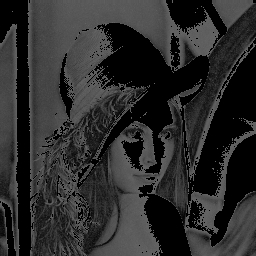
\includegraphics[scale=0.5]{./.Multimedia/lena_dilatated.jpg}

\caption{"Lena Dilatated"}
\label{lena_dilatated}

\end{figure}

Also is the function logarithmic transformation, that transforms all the pixel values to the form $f=k*log(pixel)$. To use it first we create the target image like in the other functions, after we call the function and save in the target object, and choose to save as image or display it.

\begin{lstlisting}
Image lena_log (256, 256, 1, 1, 168);
	
lena_log=lena.log_transformation();

lena_log.display("lena log");
    
lena_log.save("lena_log.jpg");
\end{lstlisting}

The logarithmic image can looks like the figure 
\ref{lena_log}

\begin{figure}[H]

\centering
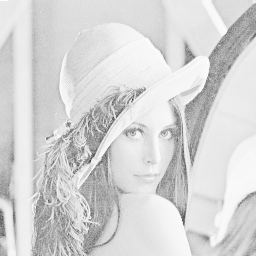
\includegraphics[scale=0.5]{./.Multimedia/lena_log.jpg}

\caption{"Lena Logarithmic"}
\label{lena_log}
\end{figure}

Other of our dot to dot transformations is the Power Law Transformation, this function transforms the pixel values to the form $f=k*pixel^gamma$, with gamma a parameter of type double, that the user gives to the function. To use it we create the target image, after we call the function specifying the order (gamma), and save or display it.

\begin{lstlisting}
Image lena_power (256, 256, 1, 1, 168);
	
lena_power=lena.power_law_transformatiom(1.1);
    
lena_power.display("lena_power");
    
lena_power.save("lena_power_law.jpg");
\end{lstlisting}

And the result can looks like the figure
\ref{lena_pow}


\begin{figure}[H]

\centering
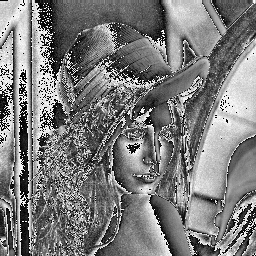
\includegraphics[scale=0.5]{./.Multimedia/lena_power_law.jpg}

\caption{"Lena Power Law"}
\label{lena_pow}
\end{figure}

The last of our dot to dot transformations is the color slicing, in this function the pixel values between  color1 and color2 set the new pixel value same as the original, and the other pixels set to the neutral color(in ths function color1 must be lower than color2). First we define the target image and the parameters color1, color2 and neutral (these parameters are arrays because if the imaga spactrum is more than 1, we need to define the colors in all the layers), after we call the function, and save/display the image.

\begin{lstlisting}
Image lena_color_slicing (256, 256, 1, 1, 168);
		
unsigned char color1[]={23};
unsigned char color2[]={130};
unsigned char neutral[]={50};
lena_color_slicing=lena.color_slicing(color1,color2,neutral);
lena_color_slicing.display("Lena Color Slicing");
lena_color_slicing.save("lena_color_slicing.jpg");
\end{lstlisting}

The result can looks like the figure
\ref{lena_color_slicing}


\begin{figure}[H]

\centering
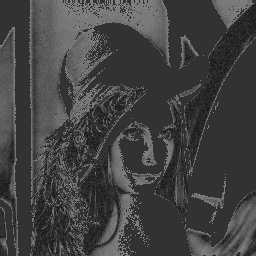
\includegraphics[scale=0.5]{./.Multimedia/lena_color_slicing.jpg}

\caption{"Lena Color Slicing"}
\label{lena_color_slicing}
\end{figure}

\end{document}